\documentclass{article}
\usepackage[margin=1.5in,includefoot]{geometry}
\usepackage{fancyhdr}
\usepackage{graphicx}
\usepackage{float}
\pagestyle{fancy}
\fancyhead{}
\fancyfoot{}
\fancyfoot[R]{\thepage\ }

\begin{document}

\begin{titlepage}

	\begin{flushleft}
	\textsc{\Large{Pontificia Universidad Catolica de Chile
	Exploratorio de Computacion}}\\
	[7cm]
	\end{flushleft}

	\begin{center}
	\line(1,0){300} \\
	[5mm]
	\huge{\bfseries{Tarea Chica 1}} \\
	[1mm]
	\line(1,0){200} \\
	[7cm]
	\end{center}
	
	\begin{flushright}
	\textsc{\Large{Leonardo Olivares \\
	86.451-K}}\\
	\end{flushright}
\end{titlepage}

\section{Learning the Command Line}
Como requerimiento de la Tarea, se completo el tutorial de CodeAcademy para aprender a utilizar el Command Line.
\begin{figure}[H]
	\centering
	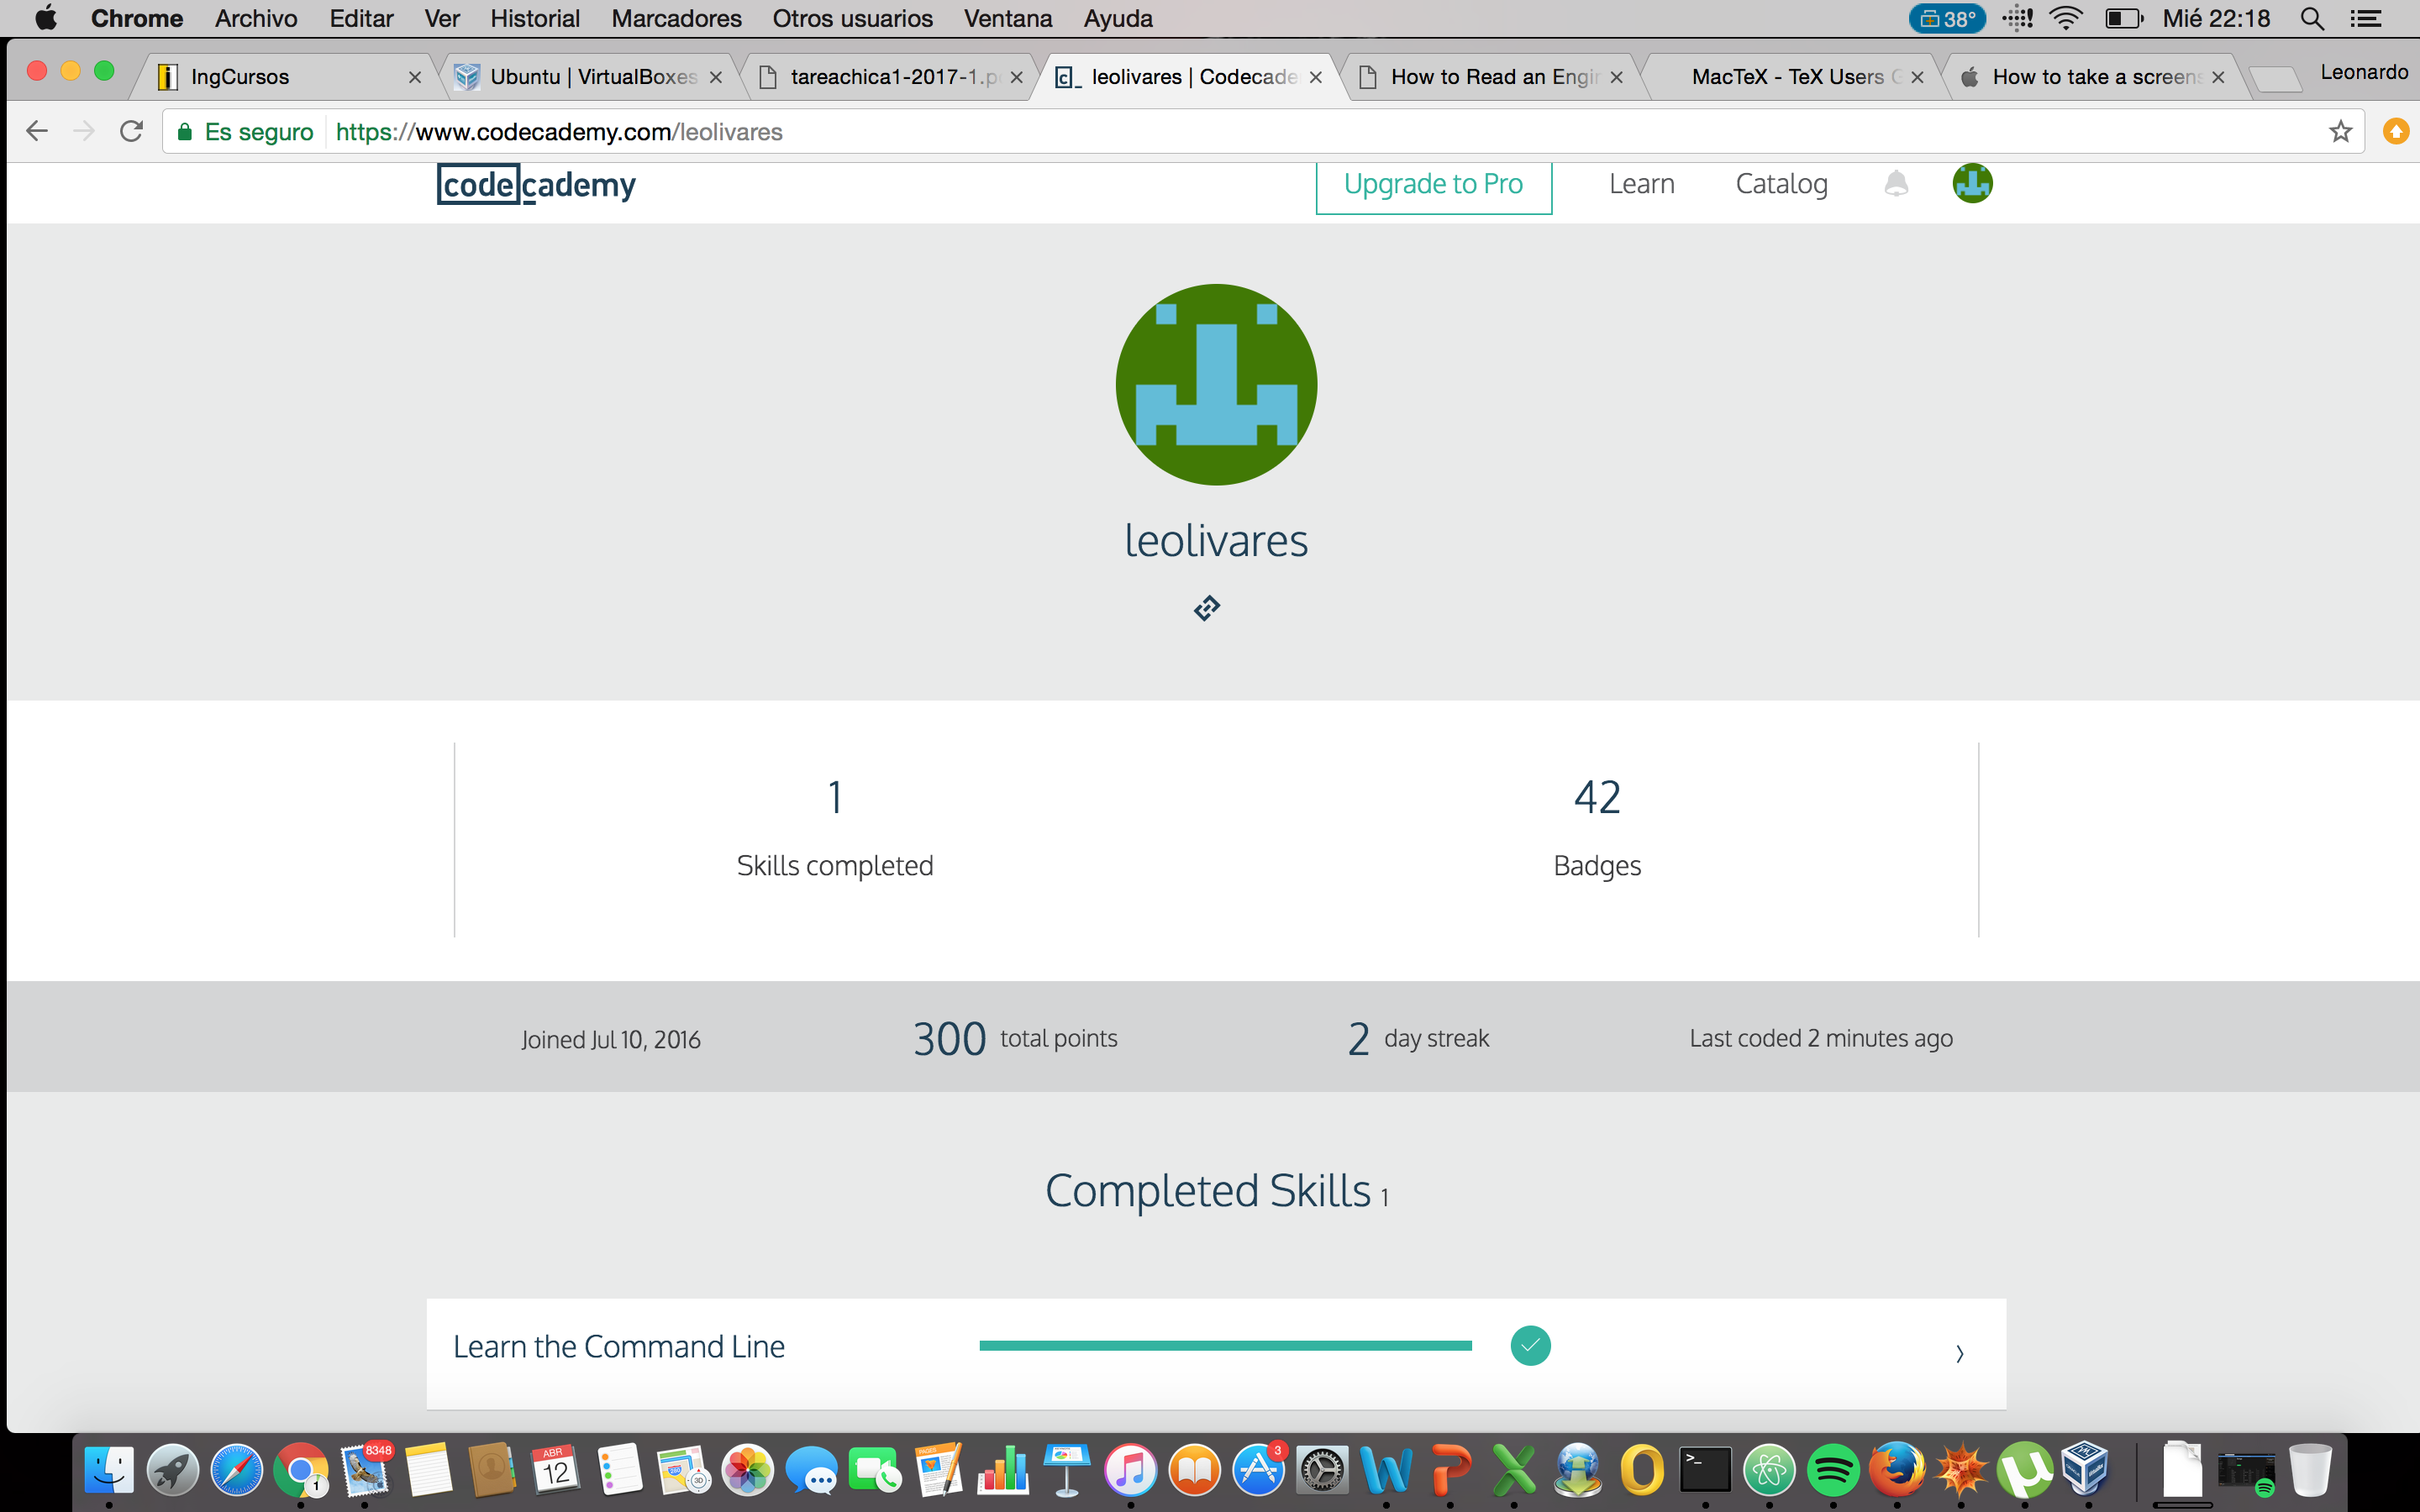
\includegraphics[width=5in,height=3in]{codeaca.png}
	\caption{Tutorial "Learning the Command Line" Completado}
\end{figure}

\section{Virtual Machine}
De igual manera, se procedio a instalar una maquina virtual (Oracle Virtual Machine), junto con una imagen de sistema operativo (en este caso, Ubuntu).
Despues, por medio de ella, se extrajeron los archivos necesarios para realizar la tarea.

Como primer paso, se cambio de directorio a TareaChica1 para leer cuales eran las intrucciones iniciales. Para esto se ejecutaron los siguientes comandos:
	\begin{itemize}

	\item{ls (Para observar que archivos tiene el directorio actual}
	\item{cd TareaChica1/  (Para cambiar de directorio al de la Tarea)}
	\item{cat primerosPasos.md  (Para mostrar el contenido del archivo en la consola)}
	
	\end{itemize}
	
\begin{figure}[H]
	\centering
	
\includegraphics[width=5in , height=3in]{1.png}
	\caption{Lectura de Primeros Pasos}
\end{figure}

Luego, se procedio a realizar lo que las instrucciones pedian. Se traslado al directorio pedido y luego se mostraron todos los archivos .txt dentro del mismo. Para esto, se utilizaron los siguientes comandos:
	\begin{itemize}

	\item{cd Carpeta\_5/SubCarpeta\_2/  (Para cambiar de directorio al mencionado en las instrucciones)}
	\item{cat *.txt  (Este comando se encarga de mostrar en consola el contenido de todos los archivos que, como unica condicion, terminen en .txt)}
	
	\end{itemize}
	
\begin{figure}[H]
	\centering
	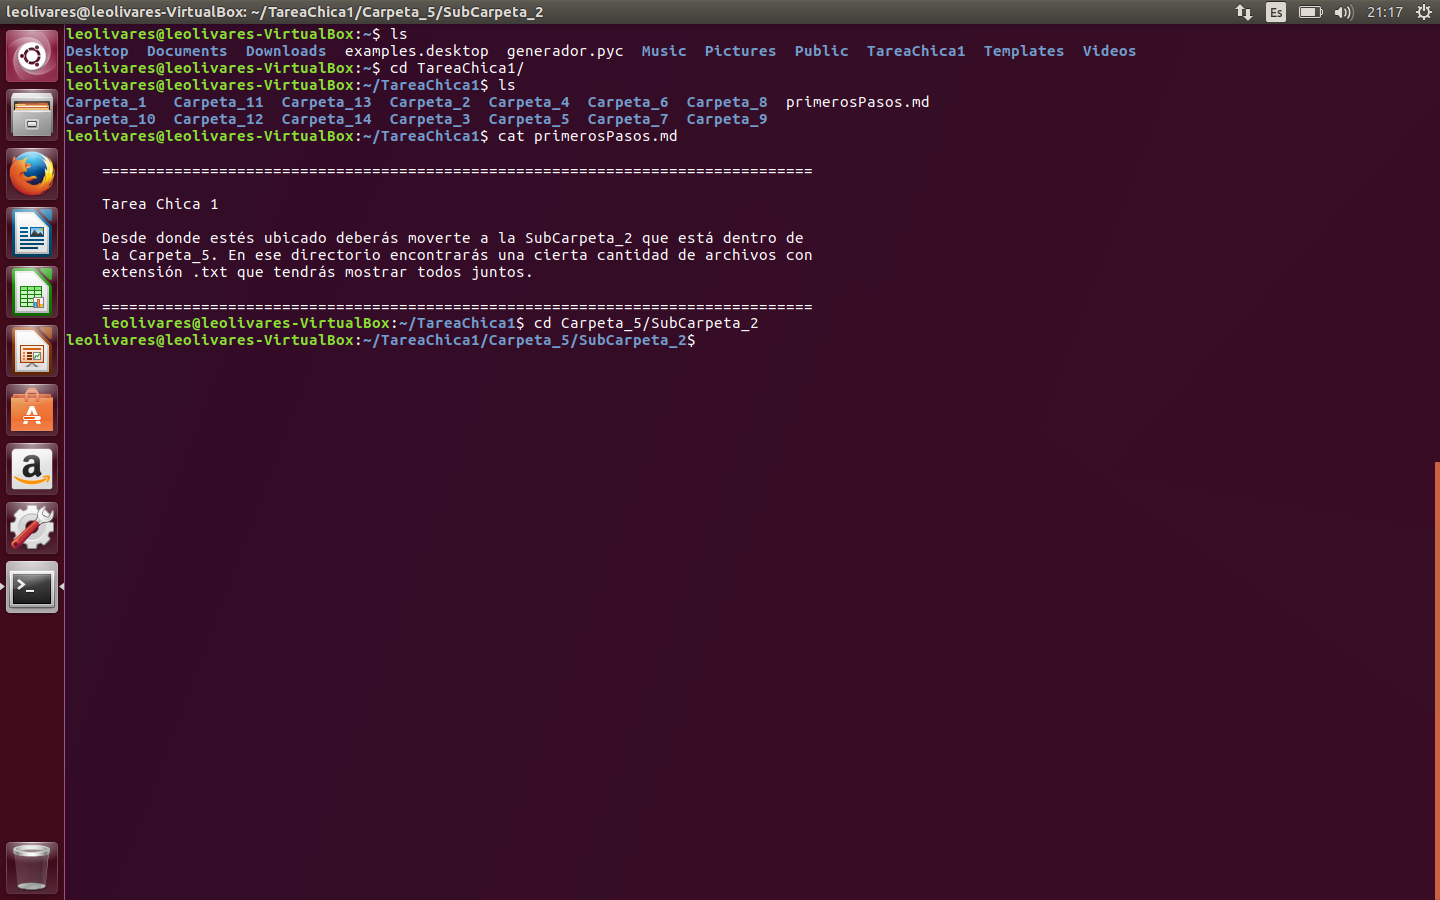
\includegraphics[width=5in , height=3in]{2.png}
	\caption{Cambiar de Directorio}
\end{figure}

\begin{figure}[H]
	\centering
	
\includegraphics[width=5in , height=3in]{3.png}
	\caption{Mostrar todos los .txt}
\end{figure}

Despues de esto, se siguieron las nuevas instrucciones. Para esto se traslado a la carpeta padre de la Tarea (que en este caso era el directorio leolivares con el path /home/leolivares), en donde se procedio a crear un nuevo directorio con el nombre LeonardoOlivares. Luego, se realizo una busqueda para todos los archivos .bla que se encontraban en la carpeta tareaChica, y se trasladaron al directorio creado recientemente. Para esto se utilizaron los siguientes comandos:

	\begin{itemize}

	\item{cd ../../../} (Para llegar al directorio padre de la Tarea)
	\item{ls}  (Para verificar que verdaderamente era el directorio padre)
	
	\end{itemize}

\begin{figure}[H]
	\centering
	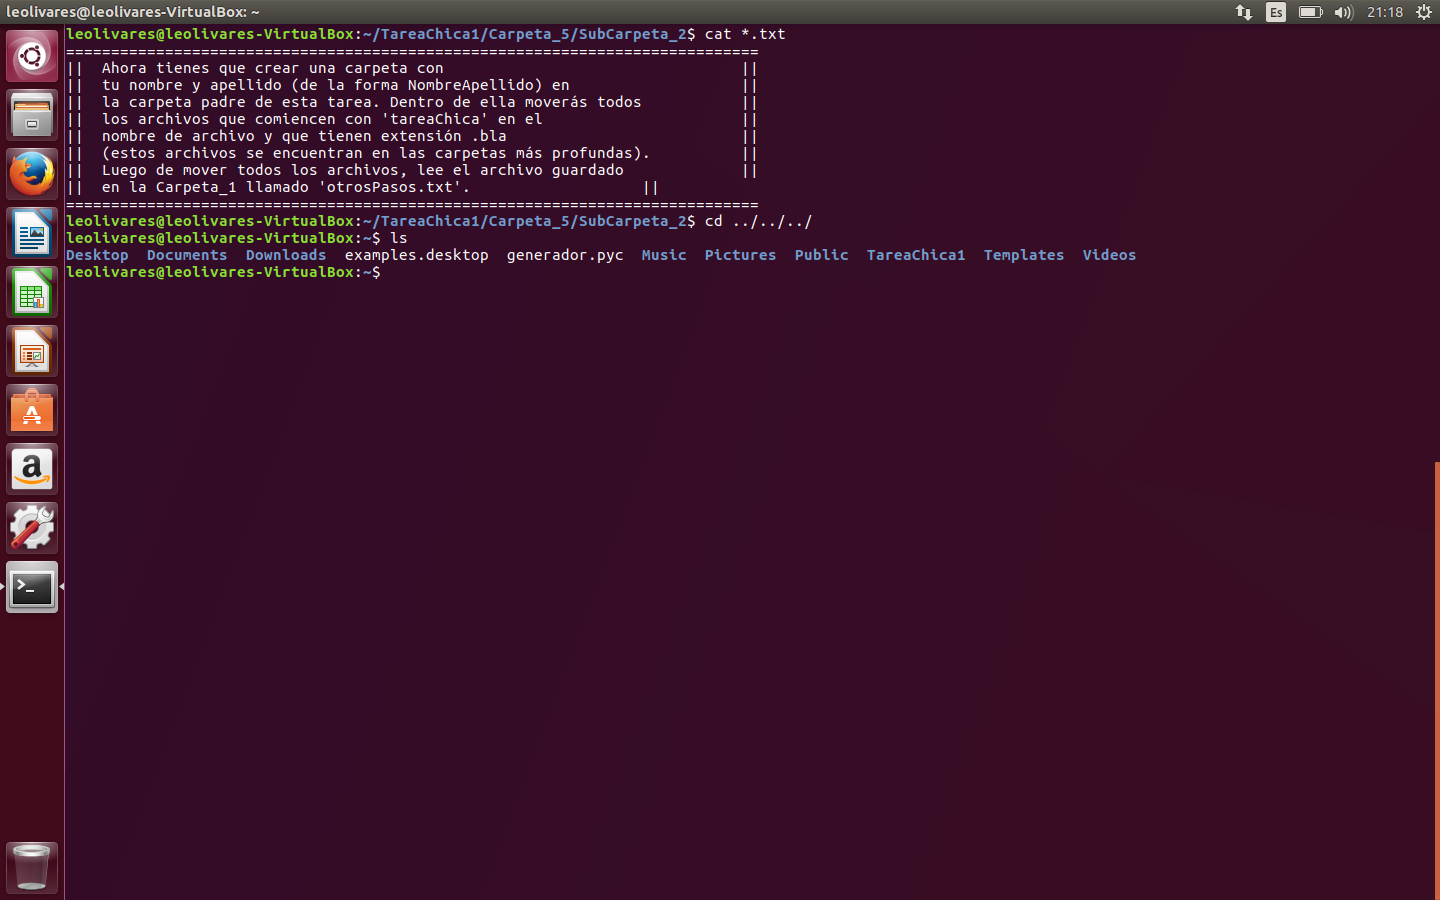
\includegraphics[width=5in , height=3in]{4.png}
	\caption{Trasladarse al directorio padre de la tarea}
\end{figure}

	\begin{itemize}

	\item{mkdir LeonardoOlivares  (Este comando crea un nuevo directorio dentro del actual con el nombre seleccionado.)}
	
	\end{itemize}

\begin{figure}[H]
	\centering
	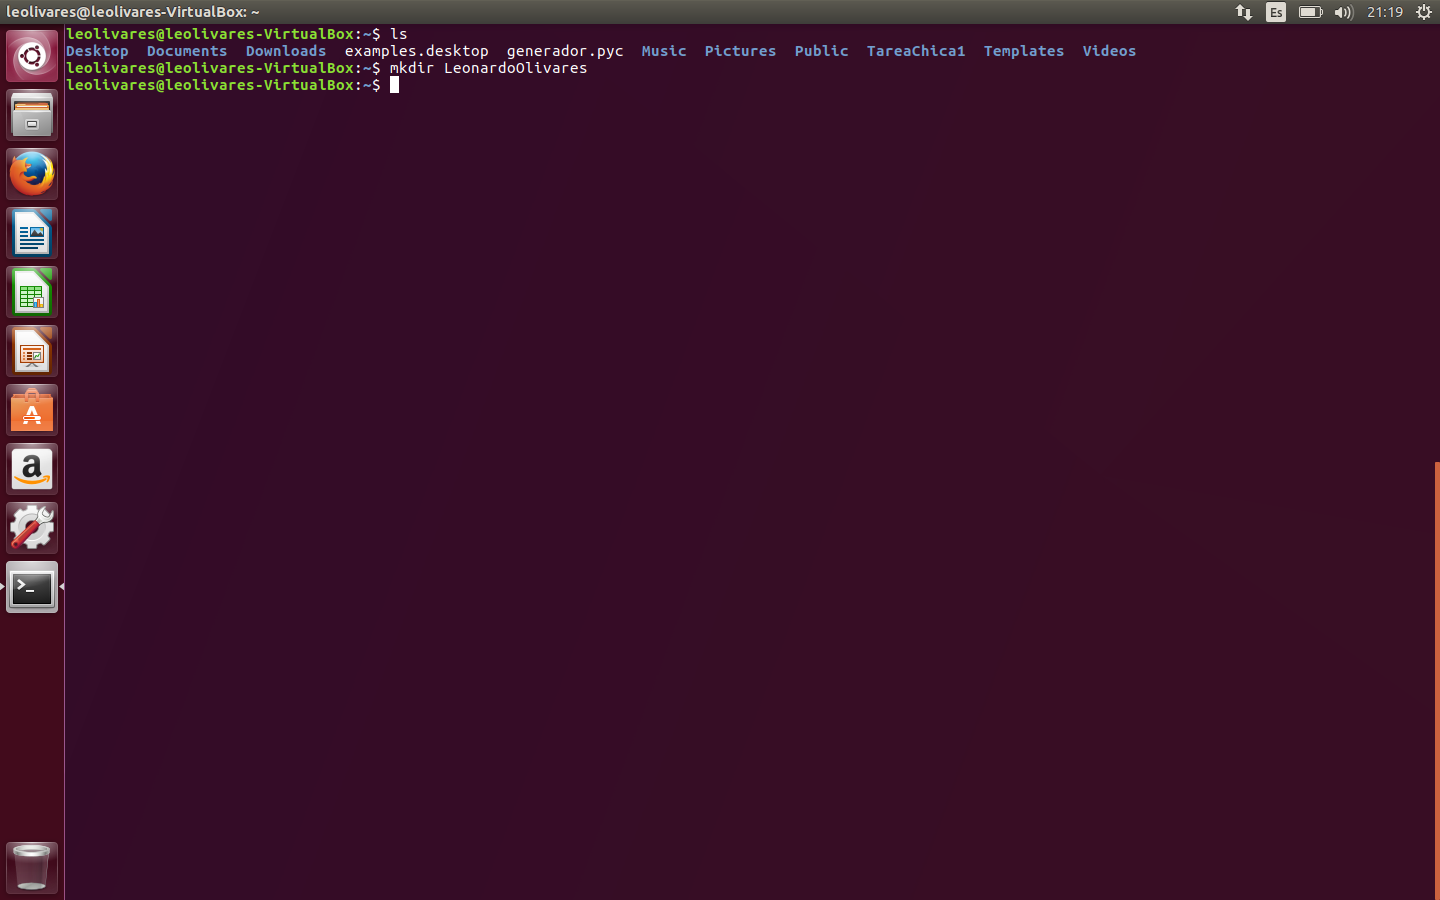
\includegraphics[width=5in , height=3in]{5.png}
	\caption{Para crear el nuevo directorio}
\end{figure}

	\begin{itemize}

	\item{find /home/leolivares/TareaChica1/ -name tareaChica*.bla -exec mv {} home/leolivares/LeonardoOlivares;}
	
	\end{itemize}
El comando find funciona de la siguiente manera. Primero se escribe el comando seguido de el path que se desea inspeccionar. Luego se agrega el nombre del archivo a buscar, en este caso se indica que el archivo debe comenzar con tareaChica pero puede culminar con cualquier otro agregado, ademas debe ser del tipo .bla. Por ultimo se agrega el comando -exec, que especifica una accion a realizar, en este caso mv, que se encarga de mover archivos de un lugar a otro. Los simbolos {} hacen referencia a los archivos obtenidos por el comando find, que pasan a entrar como parametro en mv. Por ultimo se especifica el path del directorio a donde se desean mover los archivos.
	
\begin{figure}[H]
	\centering
	
\includegraphics[width=5in , height=3in]{6.png}
	\caption{Encontrar los archivos requeridos y moverlos}
\end{figure}

	\begin{itemize}
	
	\item{ls} (Para verificar que los archivos se movieron)
	
	\end{itemize}
	
\begin{figure}[H]
	\centering
	
\includegraphics[width=5in , height=3in]{7.png}
	\caption{Verificar que los archivos de movieron}
\end{figure}

Por ultimo, se procedio a leer el archivo otrosPasos.md que se encontraba en la carpeta 1. Estas nuevas instrucciones indicaron que se buscara la cantidad de bytes en el nuevo directorio (LeonardoOlivares). Esta cantidad de bytes indicaria las coordenadas de las proximas instrucciones. Para esto, desde el directorio LeonardoOlivares se utilizo la siguiente instruccion:

\begin{figure}[H]
	\centering
	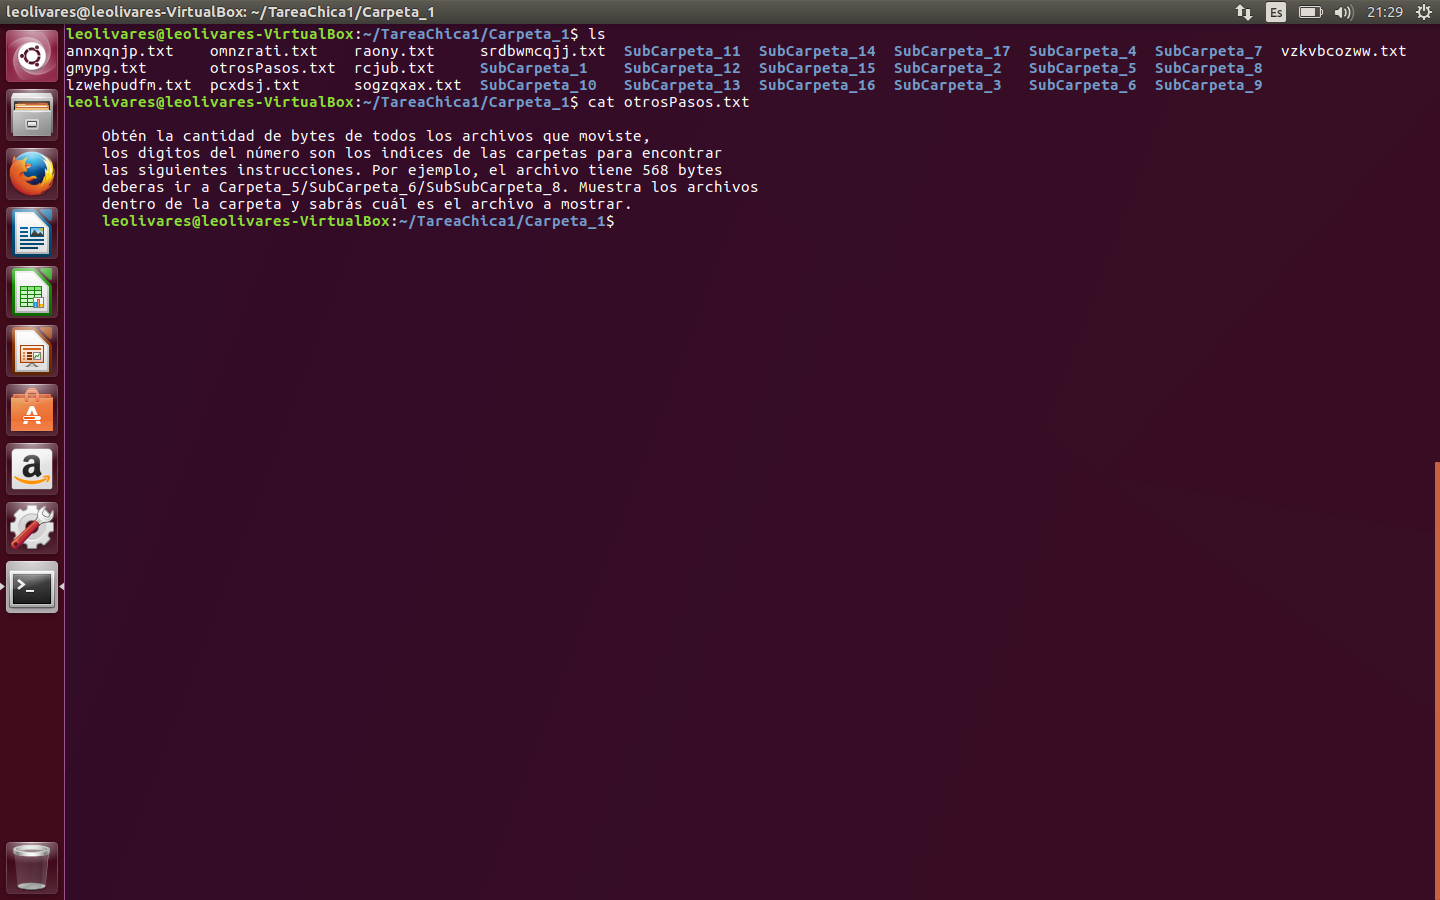
\includegraphics[width=5in , height=3in]{10.png}
	\caption{Leer otrospasos.md}
\end{figure}

	\begin{itemize}

	\item{wc -c *.bla (Este comando se encarga de entregar tama�o de cada archivo dentro de un directorio, seguido de la suma total de todos. Dicha suma es la requerida por las instrucciones.}
	\item{cd ../TareaChica1/Carpeta\_4/SubCarpeta\_4/SubSubCarpeta\_7  (Para trasladarse de el directorio actual, al obtenido con el comando anterior)}
	
	\end{itemize}
	
\begin{figure}[H]
	\centering
	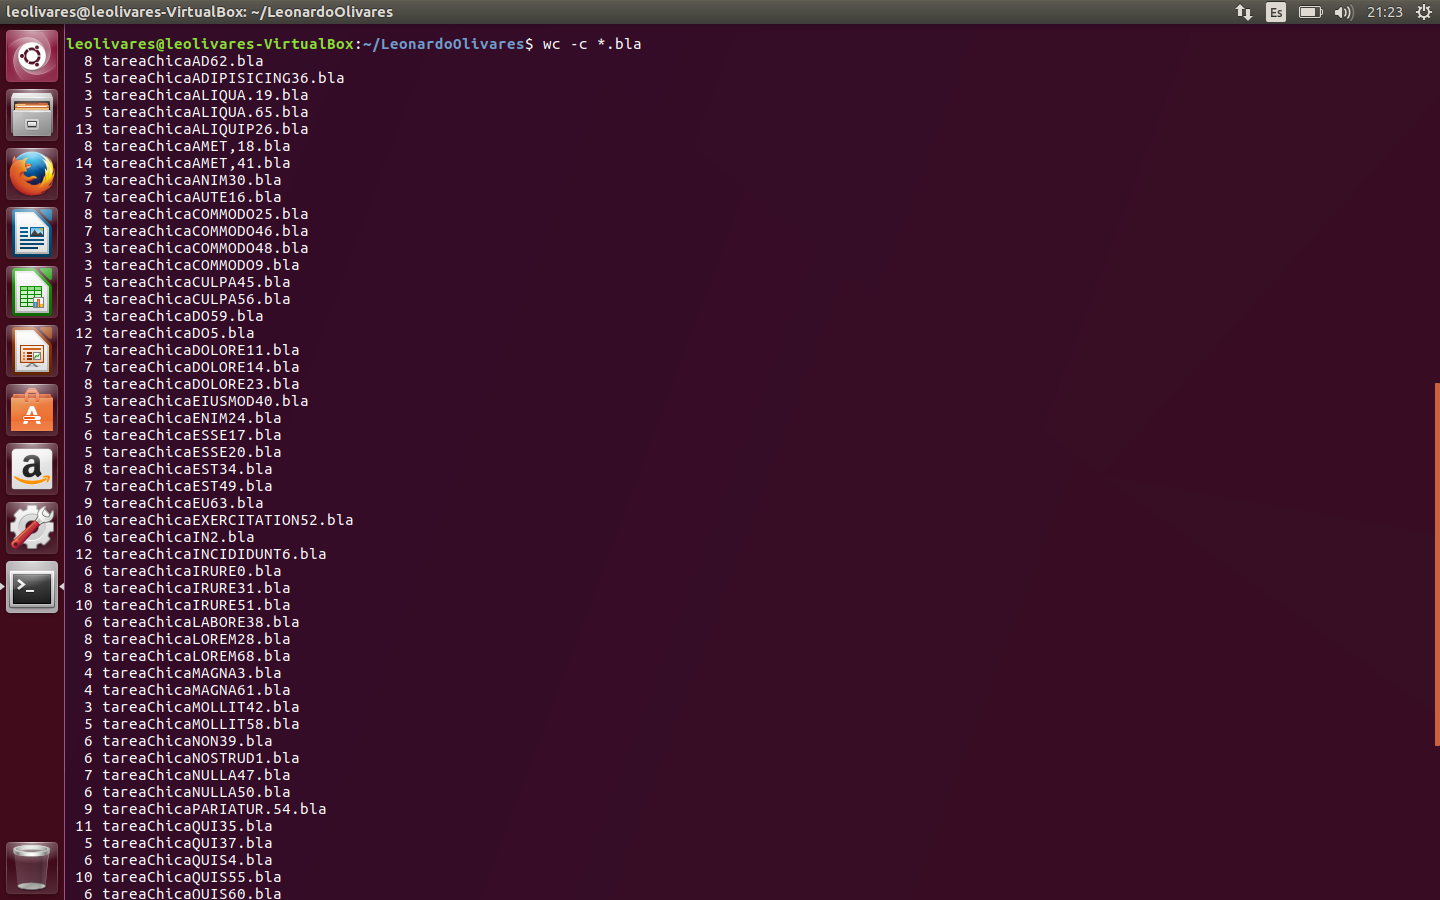
\includegraphics[width=5in , height=3in]{8.png}
	\caption{Conseguir la cantidad de bytes por archivo}
\end{figure}

\begin{figure}[H]
	\centering
	
\includegraphics[width=5in , height=3in]{9.png}
	\caption{Se traslada al directorio con la informacion}
\end{figure}

Una vez en el directorio, se revisan los archivos, se encuentra elFin.md, el cual se procede a mostrar con los siguientes comandos:

	\begin{itemize}

	\item{ls}
	\item{cat elFin.md (Para mostrar el archivo .md final)}
	
	\end{itemize}

\begin{figure}[H]
	\centering
	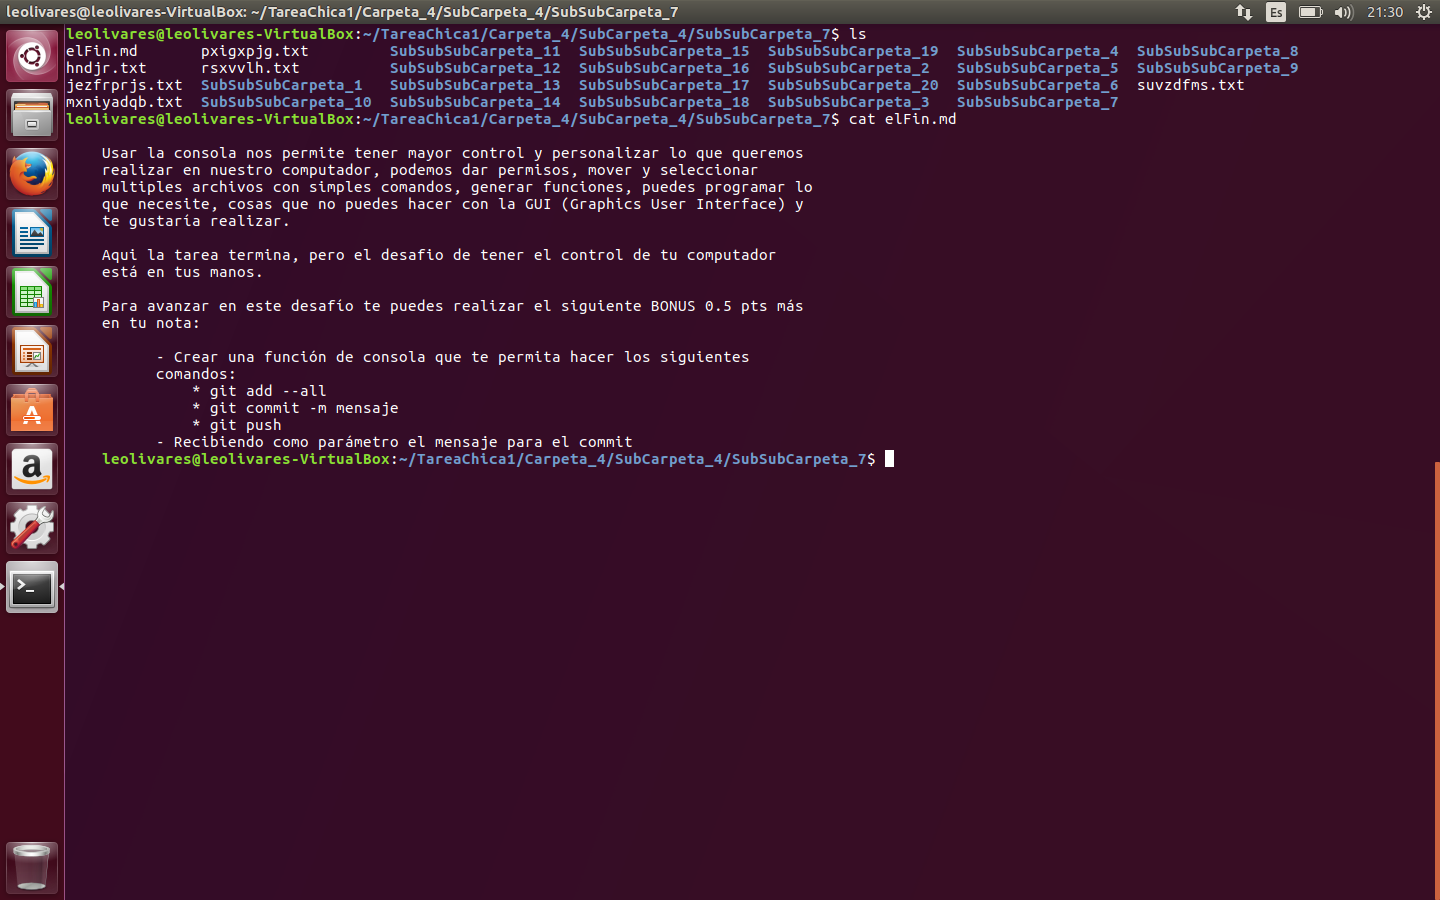
\includegraphics[width=5in , height=3in]{11.png}
	\caption{Se muestra el archivo final de la tarea}
\end{figure}

\section{BONUS}
	
Se procedio a crear una funcion por medio de command lines, la que permite a�adir todos los archivos del respectivo repositorio, luego hacer commit incluyendo un mensaje, y por ultimo realizar un push al repositorio en la pagina de github. Para esto, se modifico el archivo bash\_profile que permite agregar modificaciones como un alias, o en este caso una funcion. Entonces, los comandos utilizados para completar el bonus, fueron los siguientes:
	
	\begin{itemize}

	\item{nano \~\/.bash\_profile   (Abrimos bash\_profile para modificarlo)}
	\item{git () \{ \\
	             git add -A\\
	             git commit \$1\\
	             git push\\
	             \} }
	 \item{source \~\/.bash\_profile   (Con este comando se establecen los cambios)} 
	
	\end{itemize}
	
\begin{figure}[H]
	\centering
	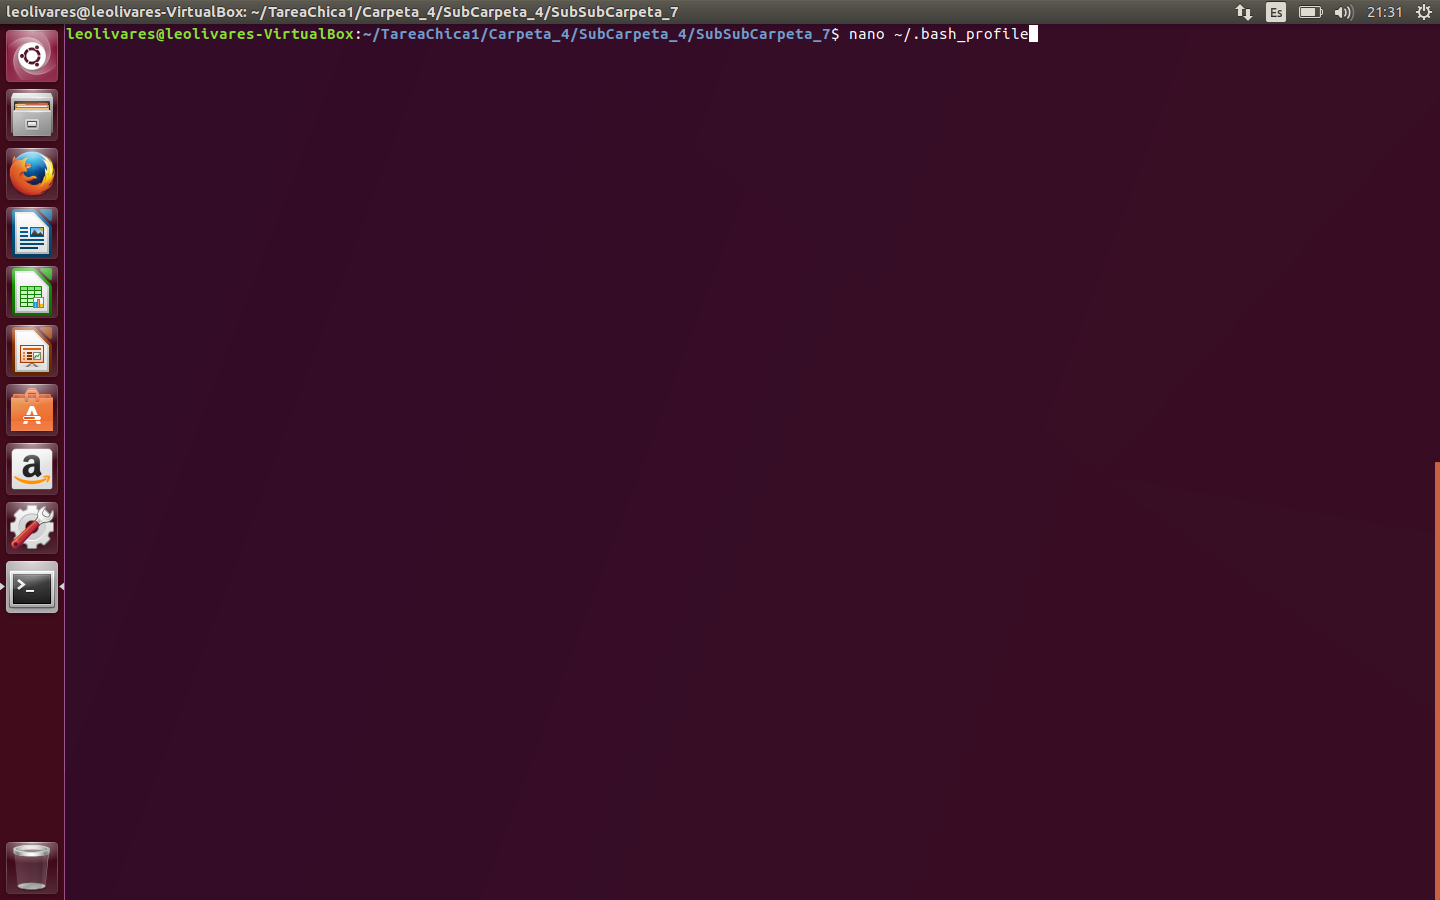
\includegraphics[width=5in , height=3in]{12.png}
	\caption{Se abre bash\_profile}
\end{figure}

\begin{figure}[H]
	\centering
	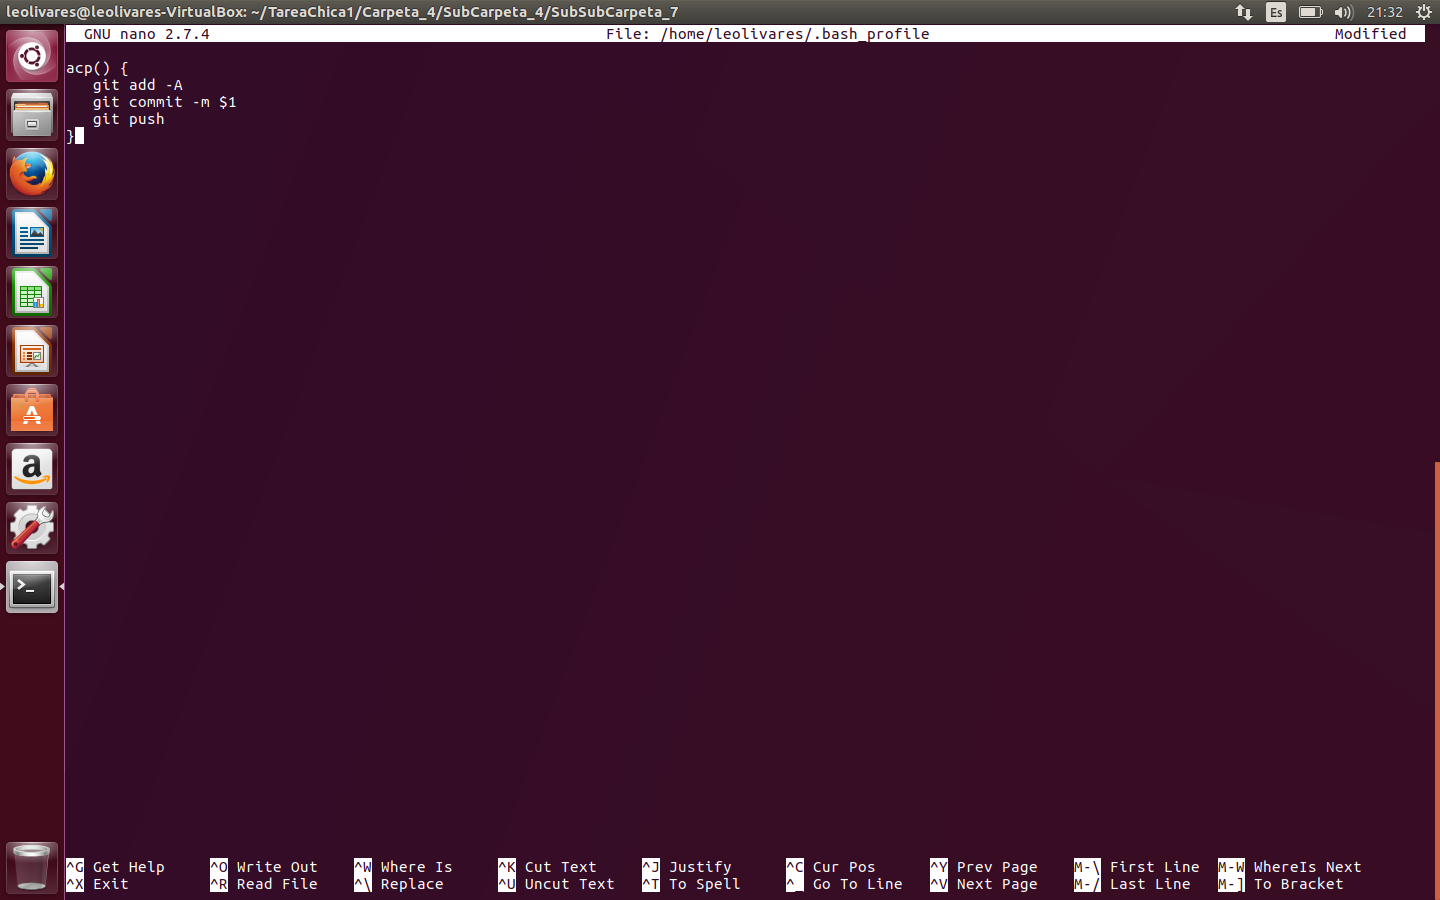
\includegraphics[width=5in , height=3in]{13.png}
	\caption{Se escribe la funcion pedida}
\end{figure}

\begin{figure}[H]
	\centering
	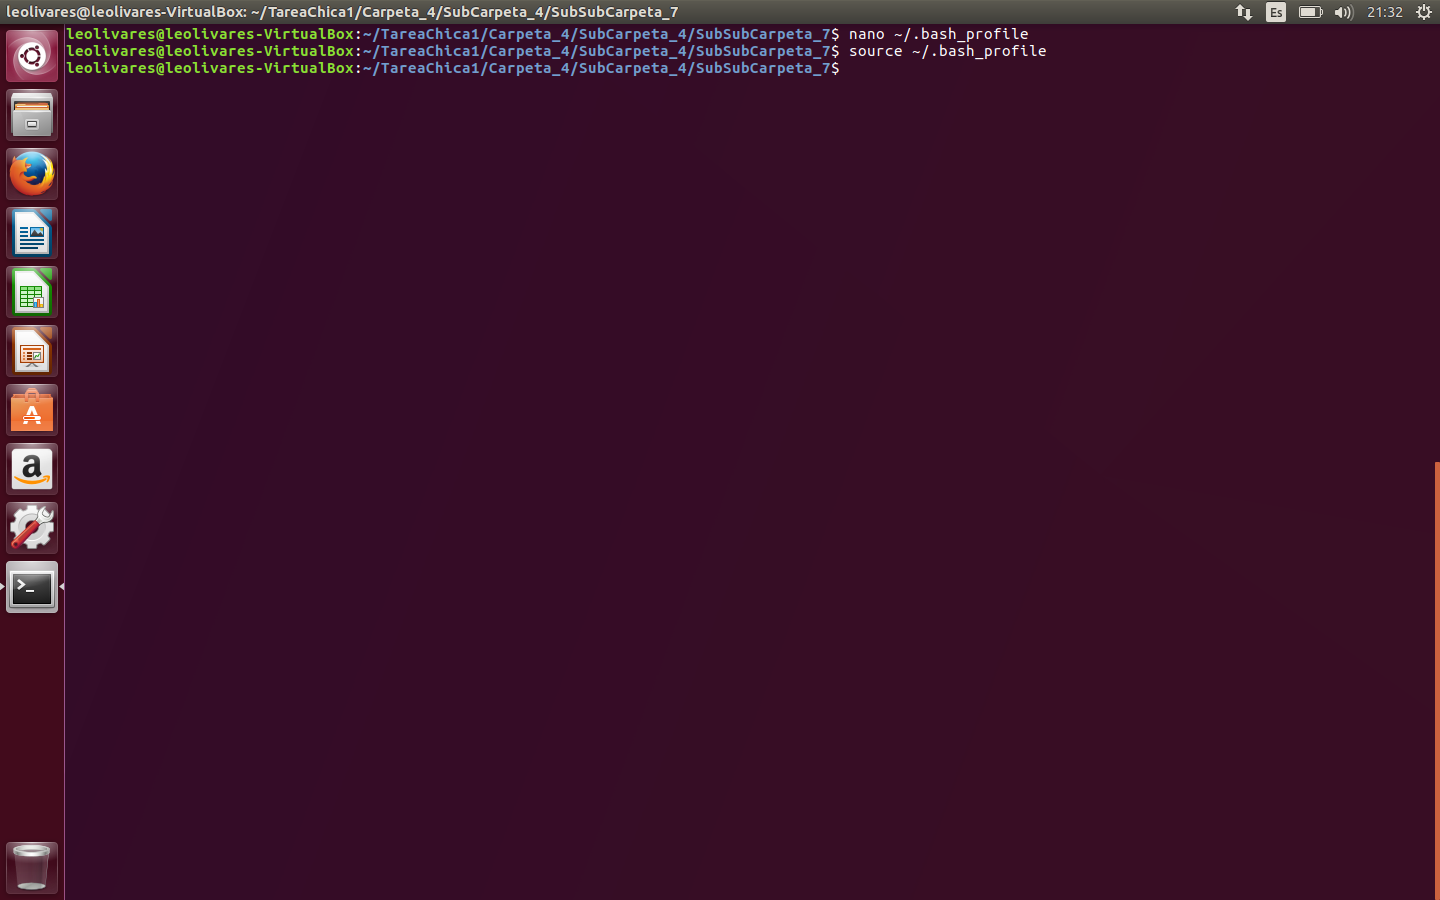
\includegraphics[width=5in , height=3in]{14.png}
	\caption{Se consolidan los cambios en la consola}
\end{figure}


Nota 1 : En la funcion, el simbolo \$1 es el parametro que en este caso es el mensaje que el usuario desea incluir al realizar el commit. Para esto, al utilizar la funcion se escribe de la siguiente manera : acp test (donde test es el mensaje a incluir en el commit y acp es la funcion).


Nota 2  : Se hizo una prueba y efectivamente los archivos deseados se subieron al repositorio de github. Para que funcione git debe estar inicializado antes en la consola, ya que las instrucciones del bonus no indicaban que la funcion debia hacerlo. Para esto, basta con escribir "git" en la consola.


\end{document}
